\section{Timed Rebeca and Floating Time Transition System} \label{sec::FTTS}

\begin{figure*}[!htbp]
 	\begin{center}
 		\small
 		\begin{mdframed}
 			\begin{align*}
 		\mathit{Model} &\Coloneqq  Class^* ~ Main \qquad \\
 				Main &\Coloneqq \mathbf{main} ~ \{ ~ InstanceDcl^* ~ \} \qquad \\
 				InstanceDcl &\Coloneqq \mathit{className} ~ \mathit{rebecName}~(\langle \mathit{rebecName} \rangle ^*)  : (\langle literal \rangle ^*);\\
 				Class &\Coloneqq \mathbf{reactiveclass} ~ \mathit{className} ~ (\mathit{queueLength}) ~ \{ ~ \mathit{KnownRebecs} ~ \mathit{Vars} ~ Constructor ~ \mathit{MsgSrv}^* ~ \}\\
 				KnownRebecs &\Coloneqq \mathbf{knownrebecs} ~ \{ ~ \mathit{VarDcl}^* ~ \} ~ \\
 				\mathit{Vars} &\Coloneqq \mathbf{statevars} ~ \{ ~ \mathit{VarDcl}^* ~ \} ~ \\
 				\mathit{VarDcl} &\Coloneqq type ~ \langle v \rangle ^+;\\
 				Constructor &\Coloneqq className ~ (\langle type ~ v \rangle ^*) ~ \{ ~ Stmt^* ~ \} \\
 				MsgSrv &\Coloneqq \mathbf{msgsrv} ~ methodName(\langle type ~ v \rangle ^*) ~ \{ ~ Stmt^* ~ \} \\
 				Stmt &\Coloneqq v = e; ~| ~ v = ?(e\langle ,e \rangle^+); ~| ~ Call;| ~ {\it if} ~ (e) ~ \{ ~ Stmt^* ~ \} ~ [else ~ \{ ~ Stmt^* ~ \}]; |  ~ \mathbf{delay}(t); \\
 				Call &\Coloneqq rebecName.methodName(\langle e \rangle ^*) ~  [\mathbf{after}(t)]  [\mathbf{deadline}(t)]
 			\end{align*}
 		\end{mdframed}
 		\caption{Abstract syntax of Timed Rebeca (adapted from \cite{DBLP:journals/scp/KhamespanahSSKI15}). Angled brackets $\langle$...$\rangle$ are used as meta parenthesis, superscript $+$ for repetition at least once, superscript $*$ for repetition zero or more times, whereas using $\langle$...$\rangle$ with repetition denotes a comma separated list. Brackets $[...]$ indicates that the text within the brackets is optional. Identifiers $className$, $rebecName$, $methodName$, $queueLength$, $v$, $literal$, and $type$ denote class name, rebec name, method name, queue length, variable, literal, and type, respectively; and $e$ denotes an (arithmetic, boolean or nondetermistic choice) expression.
 		%
 		In the instance declaration (rule $InstanceDcl$), the list of rebec names $(\langle \mathit{rebecName} \rangle ^*)$ passed as parameters denotes the known rebecs of that instance, and the list of literals $(\langle literal \rangle ^*)$ denotes the parameters of its constructor.
 		%\Ehsan{Note that $\mathit{queueLength}$ in the declaration of a reactive class,  is an integer  which specifies the queue length of this actor type. Also, in the instance declaration of rule $\mathit{InstanceDcl}$, a list of $\mathit{rebecName}$s is passed to assign to the known rebecs of that instance and a list of $\mathit{literal}$s is passed as the parameters of its constructor.}
 		%\fixme{Add the part about queue length and parameters to the constructor - Check that the syntax is consistent in the three model that we have.}
 		% \Ehsan{I added constructor definition and queue size to the syntax. Is it what you think about? or you wanna talking about semantics in the caption?}
 		 }
 		\label{fig::TRebecaSyntax}
 	\end{center}
 \end{figure*}
\begin{comment}
\begin{figure}[!htbp]
 	\begin{center}
 		\small
 		\begin{mdframed}
 			\begin{align*}
 				\mathit{Model} &\Coloneqq  Class^* ~ Main \qquad \\
 				Main &\Coloneqq \mathbf{main} ~ \{ ~ InstanceDcl^* ~ \} \qquad \\
 				InstanceDcl &\Coloneqq \mathit{className} ~ \mathit{rebecName}~(\langle rebecName \rangle ^*) \\
 							& ~~~ : (\langle literal \rangle ^*);\\
 				Class &\Coloneqq \mathbf{reactiveclass} ~ className ~ \{ \\
 					  &\ ~~~ ~ \mathit{KnownRebecs} ~ \mathit{Vars} ~ \mathit{MsgSrv}^* ~ \}\\
 				KnownRebecs &\Coloneqq \mathbf{knownrebecs} ~ \{ ~ \mathit{VarDcl}^* ~ \} ~ \\
 				\mathit{Vars} &\Coloneqq \mathbf{statevars} ~ \{ ~ \mathit{VarDcl}^* ~ \} ~ \\
 				\mathit{VarDcl} &\Coloneqq type ~ \langle v \rangle ^+;\\
 				MsgSrv &\Coloneqq \mathbf{msgsrv} ~ methodName(\langle type ~ v \rangle ^*) ~\\
				             &\ ~~~  \{ ~ Stmt^* ~ \} \\
 				Stmt &\Coloneqq v = e; ~| ~ v = ?(e\langle ,e \rangle^+); ~| ~ Call;| ~ \\
 					 &\ ~~~  ~ {\it if} ~ (e) ~ \{ ~ Stmt^* ~ \} ~ [else ~ \{ ~ Stmt^* ~ \}]; |   \\
					 &\ ~~~ ~ \mathbf{delay}(t); \\
 				Call &\Coloneqq rebecName.methodName(\langle e \rangle ^*) \\
 					 &\ ~~~  [\mathbf{after}(t)]  [\mathbf{deadline}(t)]\\
			%\\
			%	& \text{(a) Abstract Syntax of Rebeca}
 			\end{align*}
 		\end{mdframed}
 		\caption{Abstract syntax of Timed Rebeca (from \cite{DBLP:journals/scp/KhamespanahSSKI15}). Angled brackets $\langle$...$\rangle$ are used as meta parenthesis, superscript $+$ for repetition at least once, superscript $*$ for repetition zero or more times, whereas using $\langle$...$\rangle$ with repetition denotes a comma separated list. Brackets $[...]$ indicates that the text within the brackets is optional. Identifiers $className$, $rebecName$, $methodName$, $v$, $literal$, and $type$ denote class name, rebec name, method name, variable, literal, and type, respectively; and $e$ denotes an (arithmetic, boolean or nondetermistic choice) expression.
 		\fixme{Add the part about queue length and parameters to the constructor - Check that the syntax is consistent in the three model that we have}}
 		\label{fig::TRebecaSyntax}
 	\end{center}
 \end{figure}
\end{comment}

Floating Time Transition System (FTTS) is proposed based on the isolation of timed rebecs \cite{DBLP:conf/facs2/KhamespanahSVK15,DBLP:journals/scp/KhamespanahSSKI15}. The idea behind FTTS is similar to partial order reduction (POR) but the technique does not fit exactly in the definition of POR. 
%
In POR we exploit the commutativity of concurrently executed transitions, which result in the same state when executed in different orders. So, we can only expand a representative subset of all enabled transitions and abstract the rest away while preserving the properties of interest. %This way the properties are preserved. 
%
If we consider the standard Timed Transitions System semantics (TTS) of Timed Rebeca, we cannot say that FTTS is derived from TTS by POR, because we are not only abstracting away some of the transitions we are also changing the states. You cannot necessarily find one state in FTTS which is the same as a state in TTS. Both states and transitions are changed while the order of events are preserved (you may see the proof of property preservation in \cite{DBLP:conf/facs2/KhamespanahSVK15}).
%

What we mean by floating time is that in each state of the state space, different actors do not necessarily have the same local clock, i.e.,  actors are not synchronised on their local time in the state space. We consider this as letting the time \textit{float} across the actors in the state space. 
To avoid confusion, it is important to note the different models in different levels of abstraction, and also layering of models. We have (1) distributed systems, we use (2) Timed Rebeca to model distributed systems, and we model (3) the state space as Floating Time Transition System to do the analysis. 
%
Note that at the level of Timed Rebeca, actors have synchronised local clocks which gives us a notion of global time across the model. We use time stamps, and time stamps are comparable across all actors in the model. This makes our model simpler and more understandable, and our analysis more efficient.
But in distributed systems we cannot assume synchronised clocks and time stamps for distributed software components, at least not for free\footnote{Ptides\cite{DBLP:conf/dsrt/DerlerLM08} and Spanner\cite{Corbett:2013:SGG:2518037.2491245} are two examples that assume synchronized clocks  (up to an error bound) and use logical time stamps.
They proposed certain mechanisms to be able to have such assumption.}. 
For that assumption to be valid and faithful enough to the system,  we rely on the layering and different responsibilities for different layers. For distributed actors (as faithful representatives of distributed software components) to be able to have synchronised clocks and comparable time stamps we rely on the lower-level network protocols to provide that for us. 

In Timed Rebeca we have a concept of time and we can consider that each statement is executed at a certain point in time. Note that we are now talking at the level of the Rebeca model, the notion of time is the model time, and we do not need to worry about synchronising the clocks among different components in the distributed system (which are modeled as actors in our Rebeca model). We assume that local clocks of actors are synchronised and we  have time stamps on each statement  in the actors which are comparable across the actors.

In Timed Rebeca models, we use a \texttt{delay(t)} statement to show the computation delay. Other statements are assumed to be executed in zero time. We use  \texttt{after(t)} in combination with a \texttt{send} message statement, it means that the time stamp of the message when it is put in the queue of the receiver is the value of the local clock of the sender (\texttt{now} in the sender) plus the value of \texttt{t}.
The progress of time is forced by the \texttt{delay} statement and also by \texttt{after}. 
We can assume that the time stamp of all the statements are zero when a model starts to execute, then in each actor the local time is increased by value of \texttt{t} if there is a \texttt{delay(t)} statement.
A \texttt{send} statement with an  \texttt{after} does not cause any increase in the local time per se. The statement following the \texttt{send} statement has the same time stamp as the \texttt{send} statement itself.
The \texttt{after} construct may cause an increase in the time when the actor picks the message annotated by \texttt{after} to be executed. The local time of the receiver actor is set to the time stamp of the message, unless it is already greater than that.
The latter situation means that the message  sits in the queue while the actor is busy executing another message.
Remember that messages are executed atomically and are not preempted.
%
The progress of time happens in the case that the time stamp of the message is greater than the local time of the receiver actor, the local time will be pushed forward.
%
The \texttt{after} construct can be used to model the network delay, and also to model periodic events.


If we use the standard Timed Transition System (TTS) to generate the state space for Timed Rebeca model we distinguish three types of transitions: $\tau$ transitions, \textit{events}, and \textit{timed} transitions.
In FTTS we reduce that to only \textit{events} transitions.
%
We explain TTS and FTTS for Timed Rebeca using an example in Listing \ref{src::FTTS-actor-model}.
Listing \ref{src::FTTS-actor-model} shows a simple Rebeca model with two rebecs $r1$ and $r2$ instantiated from two reactive classes $RC1$ and $RC2$.
$RC1$ has only one message server ($m1$) in which it triggers the two message servers of $RC2$ ($m2$ and $m3$).
The two message servers of $RC2$ are event handlers that do nothing, i.e., there are no internal actions caused by statements like assignments, or \texttt{send}, and no  \texttt{delay} statements. Note that \texttt{send} statements are considered as internal or silent actions but they cause a change in the message queue of the receiver by adding the sent message to that queue.
 \vspace{0.5cm}

\begin{lstlisting}[language=rebeca, caption= A simple Timed Rebeca model with two rebecs, label=src::FTTS-actor-model]
reactiveclass RC1 (3) {
	knownrebecs {
		RC2 r2;
	}
	RC1() {
		self.m1();
	}
	msgsrv m1() {
		delay(2); %PC = 1
		r2.m2();  %PC = 2 
		delay(2); %PC = 3 
		r2.m3();  %PC = 4
		self.m1() after (10); %PC = 5
	}
}
reactiveclass RC2 (4) {
	knownrebecs {
		RC1 r1;
	}
	RC2() { }
	msgsrv m2() { }
	
	msgsrv m3() { }
}

main {
	RC1 r1(r2):();
	RC2 r2(r1):();
}

\end{lstlisting}
 
%\fixme{I am not sure if I have to use $m1$ or $m_1$, $r1$ or $r_1$}
%\Fatem{I think you should use $m1$ and $r1$. You have Figure 2a and 2b by using the reference ref{fig::TTS} and ref{fig::FTTS}, please check me}
Figure \ref{fig::TTS} shows the TTS generated for the model in Listing \ref{src::FTTS-actor-model}. 
The constructor of $RC1$ puts the message $m_1$ in the queue of $RC1$. So, in $time=0$ we have the message $m_1$ in the queue of $r_1$ (see state $s_0$ in Figure \ref{fig::TTS}). Also, you see that the message queue of $r_2$ is empty. On the transition from $s_0$ to $s–1$ the message is taken from the queue of $r_1$, and in the state $s_1$ the method $m_1$ is ready to be executed, i.e., the Program Counter (PC) is at $m1:1$. The first statement in $m_1$ is a \texttt{delay} statement which is executed and pushes the time forward to $time=2$ in state $s_2$.
In the state $s_2$, the PC points at a $send$ statement: $r_2.m_2()$. After this statement is executed as a silent or $\tau$ statement, we move to the state $s_3$ and have the message $m_2$ in the queue of $r–2$. The message $m_2$ is shown as $(m_2(), 2, \infty)$ in which $2$ is the timestamp of the message and $\infty$ is the value of \texttt{deadline}. The message can only be taken if and when the current time of receiver is greater than or equal its timestamp. If the current time of receiver is less than the timestamp and there is no transition of types  $\tau$  or \textit{event} enabled then the time of the receiver is advanced to the value of the timestamp (transition of type \textit{time}) and only then the message can be taken.

\begin{figure}
\centering
\begin{subfigure}[b]{0.34\textwidth}
%\subfigure[TTS]{
%\label{fig::TTS}
  \centering
  \small{
   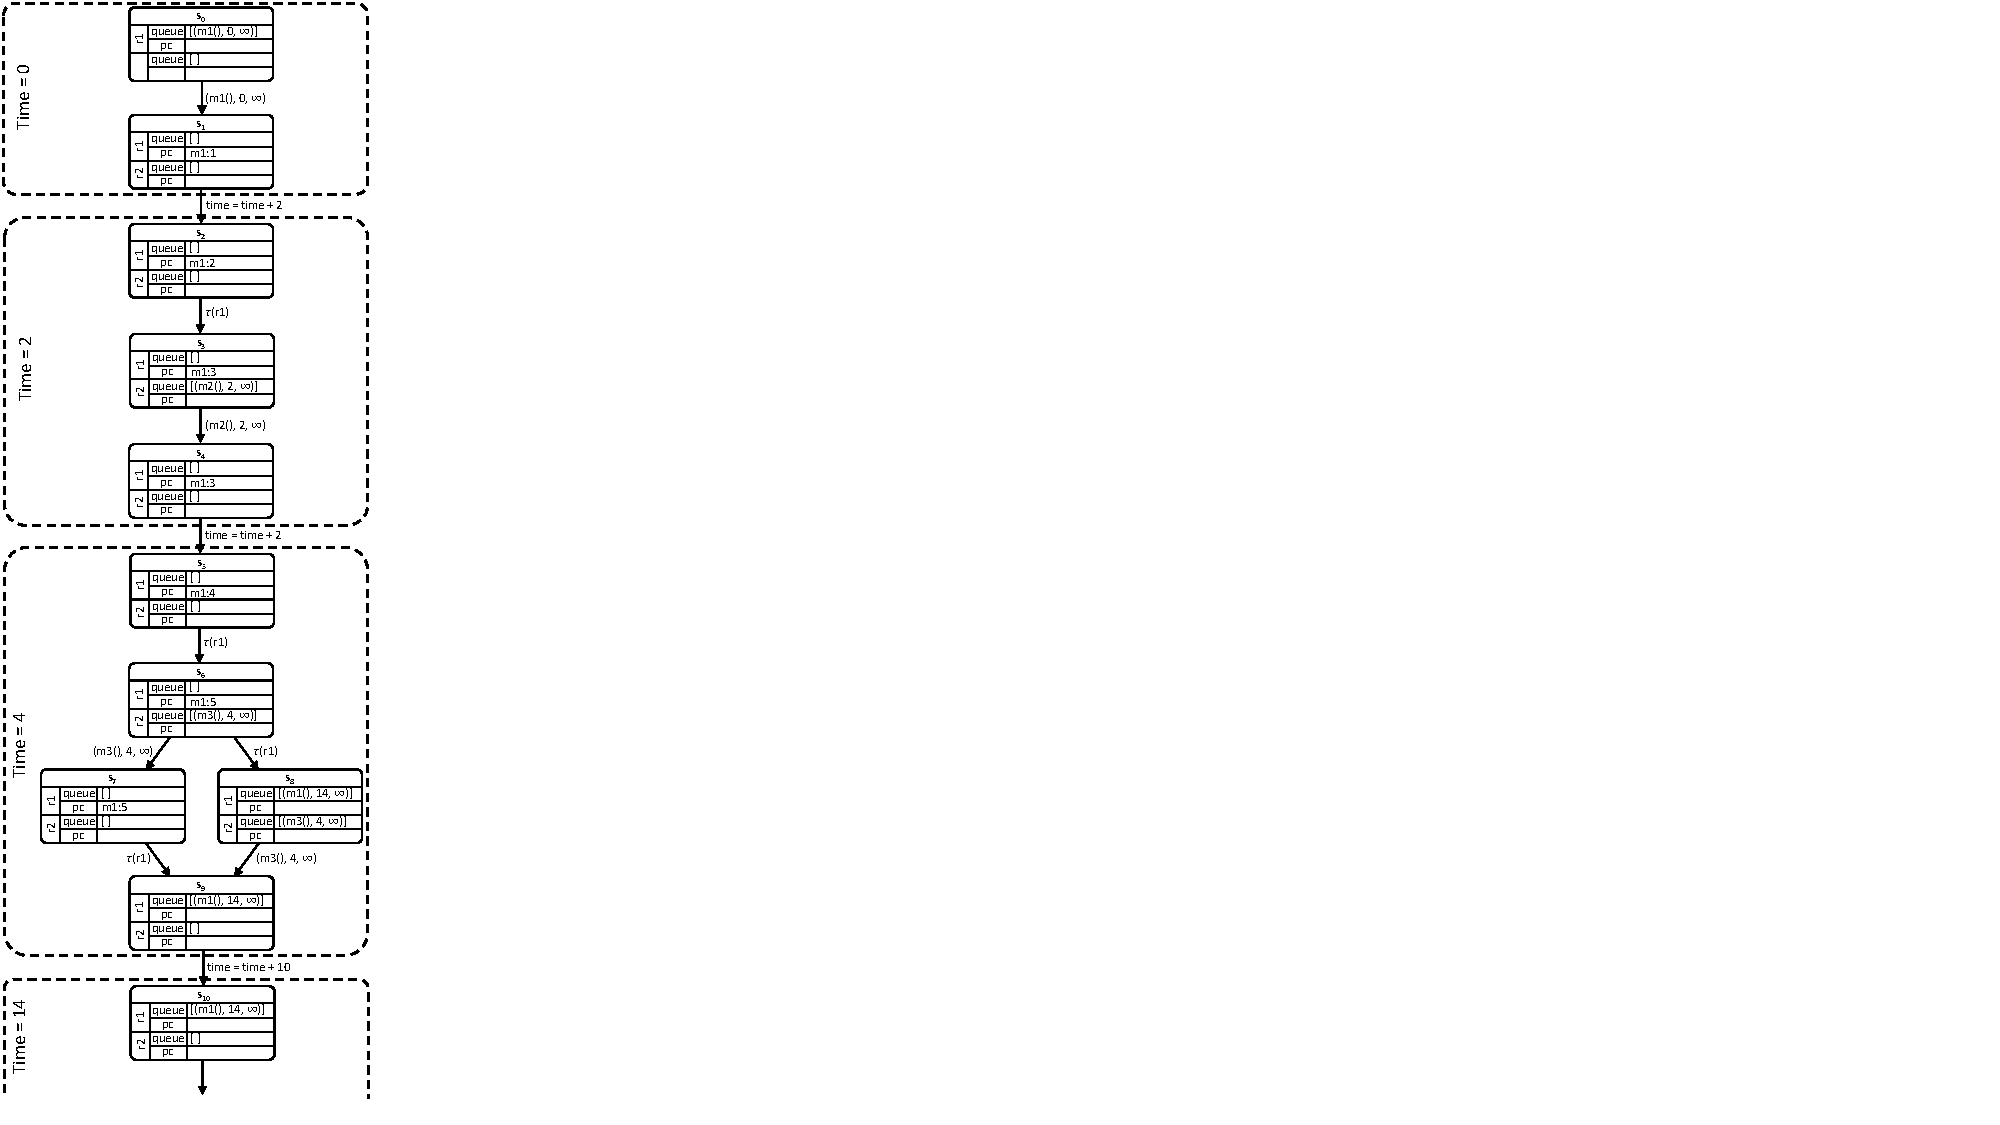
\includegraphics[width=.8\textwidth]{resources/TTS.pdf}
  }
  \caption{TTS\label{fig::TTS}}
%}
\end{subfigure}
%\qquad
\begin{subfigure}[b]{0.14\textwidth}
%\subfigure[FTTS]{
%\label{fig::FTTS}
  \centering
  \small{
   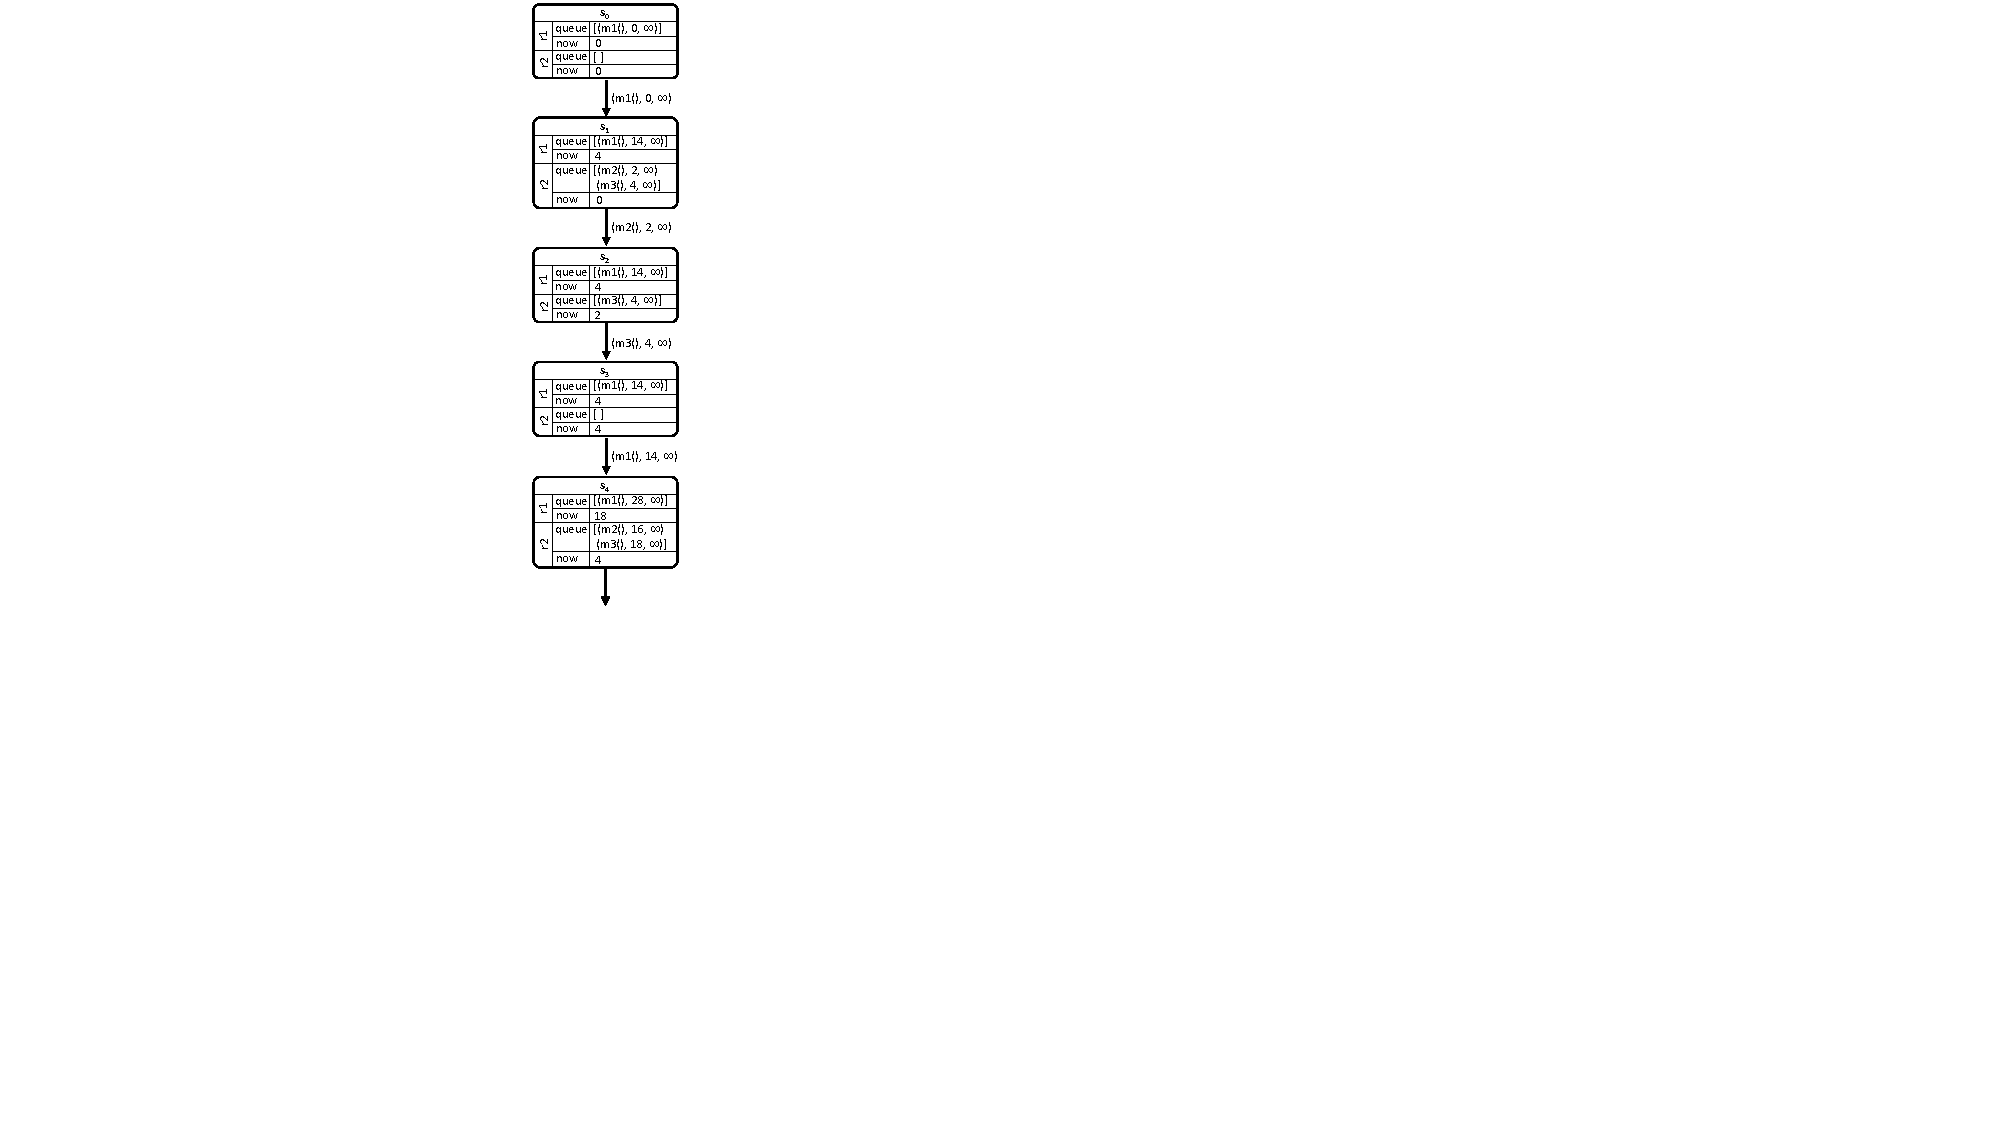
\includegraphics[width=.8\textwidth]{resources/FTTS.pdf}
   \caption{FTTS}
   \label{fig::FTTS}
  }
%}
\end{subfigure}
\caption{ TTS and FTTS for the Timed Rebeca model in Listing
\ref{src::FTTS-actor-model}.
%\fixme{Shall we add one more state to TTS such that the end transitions are the same?}
}
\label{fig::FTTSandTTS}
\end{figure}

On the transition from $s_3$ to $s_4$ the message $m_2$ is fetched to be executed, but the body of the message server $m_2$ is empty so nothing happens. We move from $s_4$ to $s_5$ by executing another \texttt{delay} statement and the time is progressed to four.
At state $s_5$ the \texttt{send} statement is executed, the message is put in the queue of $r_2$ and we will get to the state $s_6$.
At state $s_6$, two transitions are enabled and each can be  executed first non-deterministically. 
We go to the state $s_7$ if the message in the queue of $r_2$ is taken and executed first. We go to the state $s_8$ if the \texttt{send} statement at $m_1:5$  is executed first and then the message $m_1$ is put in the queue of $r_1$. No matter which trace in the diamond shown in the Figure \ref{fig::TTS} is taken, we will get to the state $s_9$.
In the state $s_8$, although there is one message in the queue of each rebec, only one transition is enabled. The reason is that   the message in the queue of $r_1$ has the timestamp of $14$ (because of the \texttt{after(10)} attached to the \texttt{send} statement).
Only in the state $s_9$, when there are no transitions of types $\tau$ or \textit{event}  enabled the transition of type \textit{time} is taken, and time is advanced for $10$ units of time. Now, at the state $s_{10}$ finally the message $(m_1(), 14,\infty )$ is enabled.

The FTTS for Listing \ref{src::FTTS-actor-model} is shown in Figure \ref{fig::FTTS}. From this figure you may observe that the only transitions in FTTS are the transitions of type \textit{event}, and you may also notice the reduction in the state space.
%
%\Marjan{I should put the following sentence somewhere appropriate.}
%In Figure \ref{fig::FTTSandTTS}.b you can see how the
Another observation is that
rebecs may have different current times (\textit{now}) in the same state. That is the reason we use the term \textit{floating time}.


%
The relation between TTS and FTTS of a Timed Rebeca model is not trivial and cannot be explained as partial order reduction, i.e., you may find states in FTTS which are not in TTS.
For example in Figure \ref{fig::FTTSandTTS} for $3$ out of $5$ states in FTTS there are no similar states in TTS. Nevertheless, in \cite{DBLP:conf/facs2/KhamespanahSVK15} we proved a bisimulation relation between FTTS and TTS to prove that the order of events is preserved in FTTS.

 It is not easy to understand the FTTS semantics of Timed Rebeca if we start from the standard TTS semantics. A better way is to start from the Timed Rebeca model, and think of an event-based semantics. By focusing on the event-based properties as the properties of interest, we narrow down the interesting transitions to the \textit{event} transitions which are taking the messages from the queue and executing the corresponding message server.
This way, we have macro-step semantics where on each transition we take the enabled event (i.e. message) and execute the corresponding message server all in one transition. This is similar to the original semantics of Rebeca presented in \cite{DBLP:journals/fuin/SirjaniMSB04}, but here we have messages in the queue tagged by timestamps (in Timed Rebeca we usually call the message queues the message bag with time-tagged messages). The main technical point here is how to choose the message to take next. The algorithm for making the state space looks into the queues of all the rebecs and picks the message that is enabled \textit{earlier} than the others.  The tricky point is to get the definition of \textit{enabled earlier} correctly. The first idea that comes to mind is to pick the message with the least timestamp, but we also need to check the current time or \textit{now} of the receiver rebec. If the value of \textit{now} is larger than the timestamp then that would be the time that the message can really be taken. So,  for each rebec we need to find the maximum between  the timestamps and the value of  \textit{now} of the receiver rebec, and we need to do that for all the rebecs and all the messages in their queues,  and find the least among these values. That would be the message that will be taken first and will be the event on the next transition. There may be more than one message with that characteristic, and in that case the choice is nondeterministic.



\begin{figure}
\centering
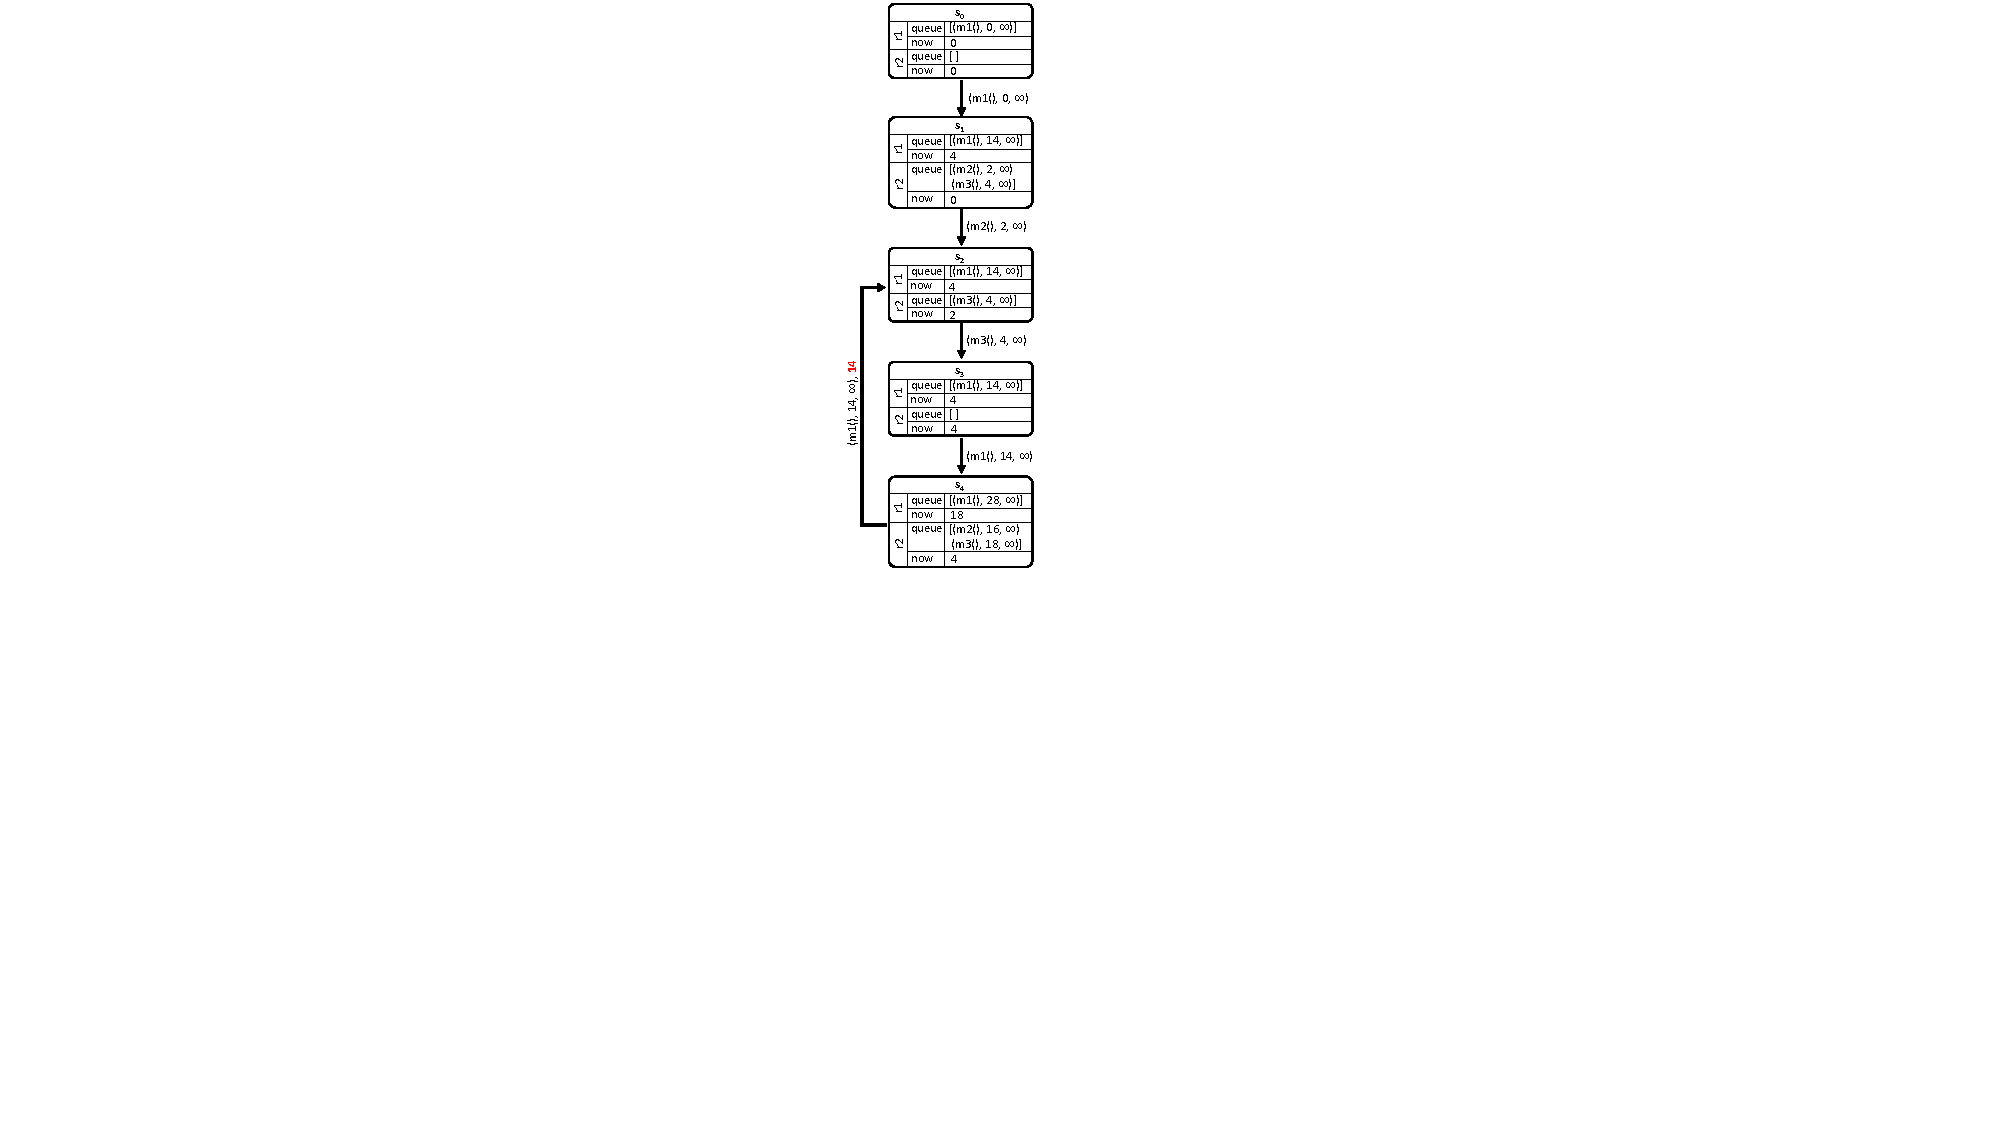
\includegraphics[width=.15\textwidth]{resources/BFTTS.pdf}
\caption{ Bounded FTTS for the Timed Rebeca model in Listing \ref{src::FTTS-actor-model}.}
\label{fig::BFTTS}
\end{figure}

The Bounded Floating Time Transition System (BFTTS) for Listing \ref{src::FTTS-actor-model} is shown in Figure \ref{fig::BFTTS}. 
In many reactive systems the behavior becomes recurrent after a while, and it gives us the chance to have a bounded number of states and transitions. When we add the notion of time to our model and consequently to the transition system, when the time is increasing in the model we are at the risk of having an unbounded %\Ehsan{infinite instead of unbounded} 
state space even when the behavior is recurrent.
In BFTTS, if the only difference between two states is an equal shift in \textit{time-dependent} values (we call it \textit{shift-equivalency}) we merge those two states to one and will make the shift clear on the transition. %\Ehsan{Note that the future behavior of these two states are the same as there is no statement in Timed Rebeca that have access to the absolute time of the model.} 
Note that this can work because there is no statement in Timed Rebeca that allows assigning an absolute value to \textit{now}, or accessing the absolute value of \textit{now} (if necessary, we may allow that but the modeler has to be careful not to break the shift-equivalency). 

We have an example of a recurrent behavior in Figure \ref{fig::BFTTS}. After state $s_4$ we move to a state which is equivalent to state $s_2$ with a shift in both now variables (to be $18$ for $r_1$  and $16$ for $r_2$), and also a shift $14$ for the time tags of the messages (to be $28$ for the message in the queue of $r_1$ and $18$ for the message in the queue of $r_2$). So, we do not create a new state, instead we put a transition back to $s_2$, and make the shift of $14$ for the \textit{time-dependent} values clear on this transition. The model checking tool of Timed Rebeca is developed using the idea of BFTTS to be able to generate bounded state spaces and it is integrated in Afra. To illustrate the efficiency of FTTS, the result of comparing the state space size and model checking time consumption of a set of Timed Rebeca examples are presented in Table~\ref{table::TTS-FTTS-experiment}.

%\Marjan{Ehsan, would you please read the above paragraph? is it correct? can you add 1-2 sentences to say how we continue from where I stopped?}

\begin{table*}
    \small
  \begin{center}
          \begin{tabular}{|l|l|c|c|c|c|c|c|c|c|}
        \hline
        & \multirow{2}*{{Config}}&\multicolumn{3}{c|}{FTTS} &\multicolumn{3}{c|}{TTS} &\multicolumn{2}{c|}{Reduction}\\
        & & States & Trans. & Time & States & Trans. & Time & States & Trans.\\
        \hline
        \multirow{5}*{{Hadoop YARN Scheduler}}
        &\textbf{1 AM} & 25 & 41 & $<1$  sec  & 132    & 148    & $<1$ sec  & 19$\%$  & 28$\%$  \\
        &\textbf{2 AMs} & 499 & 1.02K & 1  sec  & 3.01K    & 4.28K    & 1 sec  & 17$\%$  & 24$\%$  \\
        &\textbf{3 AMs} & 5.10K & 13.3K & 1  sec  & 34.3K    & 66.7K    & 1 sec  & 15$\%$  & 20$\%$  \\
        &\textbf{4 AMs} & 28.19K & 92.87K & 2 secs  & 219K    & 553K    & 7 secs  & 13$\%$  & 17$\%$  \\
        &\textbf{5 AMs} & 220K & 840K & 11 secs  & 1.94M    & 5.69M    & 70 secs  & 11$\%$  & 15$\%$  \\
        \hline
        \multirow{6}*{{WSAN Application}}
        & \textbf{33-6-4-2}  & 386 & 548 & $<1$ sec  & 1.58K & 2.69K & $<1$ sec  & 24$\%$ & 20 $\%$ \\
        & \textbf{25-6-4-2}  & 1.21K & 1.63K & $<1$ sec  &  5.04K & 8.59K & $<1$ sec & 24$\%$ & 19$\%$ \\
        & \textbf{30-6-4-2}  & 2.90K & 3.25K & $<1$ sec  & 13.00K & 20.54K & 2 secs  & 22$\%$ & 16$\%$ \\
        & \textbf{25-5-4-10} & 3.54K & 5.01K & $<1$ sec  & 19.59K & 38.61K & 2 secs  & 18$\%$ & 13$\%$ \\
        & \textbf{25-7-5-10} & 4.87K & 6.66K & $<1$ sec  & 25.42K & 48.29K & 2 secs  & 19$\%$ & 14$\%$ \\
        & \textbf{50-9-3-2} & 9.20K & 11.79K & 1 sec    & 49.33K & 91.93K & 3 secs  & 18$\%$ & 13$\%$ \\
        \hline
        \multirow{7}*{{Ticket Service System}}
        & \textbf{1 Customer} & 5     & 6     & $<1$ sec  & 13     & 16     & $<1$ secs  & 38$\%$  & 37 $\%$  \\
        & \textbf{2 Customers} & 51        & 77        & $<1$ sec  & 155        & 285       & $<1$ sec  & 33$\%$  & 27$\%$  \\
        & \textbf{3 Customers} & 252       & 418       & $<1$ sec  & 842       & 1894       & $<1$ sec  & 30$\%$  & 22$\%$  \\
        & \textbf{4 Customers} & 1.29K     & 2.21K     & $<1$ sec  & 4.75K     & 12.6K      & 1 sec     & 27$\%$  & 18$\%$   \\
        & \textbf{5 Customers} & 7.53K & 12.8K & $<1$ sec  & 29.1K & 85.9K & 2 sec  & 26$\%$  & 15$\%$   \\
        & \textbf{6 Customers} & 51.6K & 84.7K & 3 secs  & 195.3K & 599.3K  & 9 secs  & 26$\%$  & 14$\% $  \\
        & \textbf{7 Customers} & 408K  & 650K  & 11 secs  & 1.46M  & 4.34M & 67 secs  & 28$\%$  & 15$\% $  \\
        \hline
        \end{tabular}
        \end{center}
        \caption{Comparing the number of states and transitions in TTS and FTTS of three different example (from~\cite{ehsan-phd-thesis}). %\fixme{Ehsan, Dont we have larger examples where tts is impossible but ftts is possible?}
        }
\label{table::TTS-FTTS-experiment}
\end{table*}
%\fixme{Ehsan, would you please add a table for experiments of FTTS here?}
